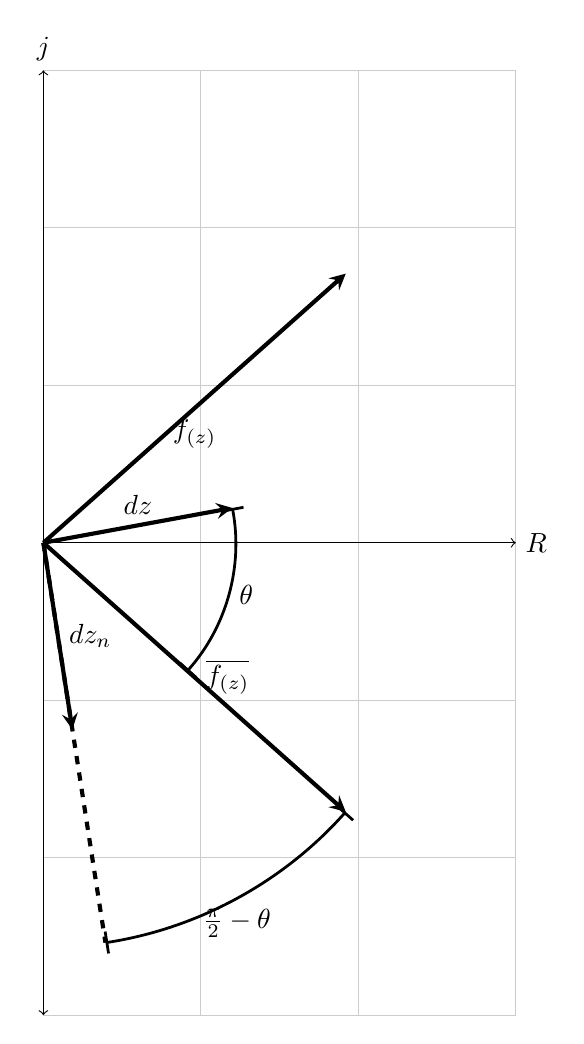
\begin{tikzpicture}[scale=2]
        \draw[thin,gray!40] (0,-3) grid (3,3);
        \draw[<->] (0,0)--(3,0) node[right] {$R$};
        \draw[<->] (0,-3)--(0,3) node[above]{$j$};
        
        \coordinate (a) at (1.6*1.2,1.424*1.2);
        \coordinate (b) at (1.6*1.2,-1.424*1.2);
        \coordinate (c) at (1*1.2,0.184*1.2);
        \coordinate (d) at (0.1533*2.57,-0.988*2.57);
        \coordinate (e) at (0.1533*1.2,-0.988*1.2);
        
       

        \draw[line width=1.5pt,-stealth] (0,0)--(a) node[midway, below]{$f_{(z)}$};
        \draw[line width=1.5pt,-stealth] (0,0)--(b) node[midway, right]{$\overline{f_{(z)}}$};
        \draw[line width=1.5pt,-stealth] (0,0)--(c) node[midway, above]{$dz$};
        \draw[line width=1.5pt,-stealth] (0,0)--(e) node[midway, right]{$dz_n$};
        \draw[line width=1.5pt,dashed] (0,0)--(d) node[midway, above]{};
        
        \draw[line width=1,|-|] (c) arc (10.67:-41.67:1.22) node[midway,right]{$\theta$};
         \draw[line width=1,|-|] (b) arc (-41.67:-81.18:2.57) node[midway,below]{$\frac{\pi}{2}-\theta$};
        
\end{tikzpicture}